\documentclass{beamer}
% Sans animations
%\documentclass[handout]{beamer}

\usepackage{tikz}
\usepackage{pgfplots}
\tikzstyle{every picture}+=[remember picture]

\setbeamertemplate{footline}[frame number]

\title{ALG4 : algorithmes de tri}
\author{}
\date{loig.jezequel@univ-nantes.fr}

\begin{document}

\frame{
\maketitle
}

\frame{
\frametitle{Context du cours}

\begin{block}{Problème général}
Étant donnée une liste d'éléments, on souhaite trier ces éléments selon un ordre donné.
\end{block}

\begin{exampleblock}{Par exemple}
Trier des mots par ordre alphabétiques, des nombres du plus petit au plus grand, des couleurs de la plus foncée à la plus claire, etc.
\end{exampleblock}

\begin{block}{Problème simplifié pour ce cours}
Étant donné un tableau d'entiers $t$ on souhaite produire un tableau $t'$ qui contient les mêmes entiers rangés du plus petit au plus grand.
\end{block}

\begin{exampleblock}{Par exemple}
si $t =$ \begin{tabular}{|c|c|c|c|c|}
\hline
12 & 32 & 7 & 23 & 9 \\
\hline
\end{tabular}
alors $t' =$ \begin{tabular}{|c|c|c|c|c|}
\hline
7 & 9 & 12 & 23 & 32 \\
\hline
\end{tabular}
\end{exampleblock}

}

\frame{
\frametitle{Solution : algorithmes de tri}

\begin{block}{Tri par insertion}
Mettre les éléments un par un, à la bonne place, dans un tableau initialement vide.
\end{block}

\begin{block}{Tri fusion}
Trier plusieurs sous ensembles d'éléments, puis les réunir en un seul tableau trié.
\end{block}

\begin{block}{Tri rapide}
Permutations d'éléments pour mettre chaque élément à la bonne place (tous les plus petits à sa gauche, tous les plus grands à sa droite).
\end{block}

\begin{block}{Et plein d'autres}
Tri à bulles, tri par tas, tri par sélection, etc.
\end{block}

}

\frame{
\frametitle{Pourquoi plusieurs algorithmes différents ?}

\begin{block}{Tri en place ou non}
Un tri est dit \alert{en place} s'il est fait directement dans la structure de donnée à trier~: il n'y a pas de recopie des données.
\end{block}

\begin{block}{Tri stable ou non}
Un tri est dit \alert{stable} s'il n'altère pas l'ordre des éléments de même valeur. Ceci n'a pas d'importance sur un tableau d'entiers, mais peut en avoir si on trie des objets plus complexes (par exemple des étudiants qu'on trie par leur nom de famille).
\end{block}

\begin{block}{Complexité dans le pire cas variable}
Nombre d'opérations nécessaires dans le pire cas pour réaliser le tri.
\end{block}

\begin{block}{Complexité en moyenne variable}
Nombre d'opérations nécessaires en moyenne pour réaliser un tri.
\end{block}

}

\frame{
\frametitle{Le tri par insertion : principe}

\begin{block}{Idée générale}
Construction d'un tableau trié un y ajoutant les entiers un à un, à la bonne place.
\end{block}

\begin{center}
\begin{tikzpicture}
\node (12) at (0.5,0.5) {12};
\node (32) at (1.5,0.5) {32};
\node (7) at (2.5,0.5) {7};
\node (23) at (3.5,0.5) {23};
\node (9) at (4.5,0.5) {9};
\draw (0,0) -- (5,0) -- (5,1) -- (0,1) -- (0,0);
\draw (1,0) -- (1,1);
\draw (2,0) -- (2,1);
\draw (3,0) -- (3,1);
\draw (4,0) -- (4,1);

\uncover<2->{
\draw (0,0) -- (1,1);
}
\uncover<4->{
\draw (1,0) -- (2,1);
}
\uncover<6->{
\draw (2,0) -- (3,1);
}
\uncover<8->{
\draw (3,0) -- (4,1);
}
\uncover<10->{
\draw (4,0) -- (5,1);
}

\uncover<2-3>{
\node (12) at (0.5,-2.5) {12};
\draw (0,-2) -- (1,-2) -- (1,-3) -- (0,-3) -- (0,-2);
}

\only<3>{
\draw[->] (1.5,0) -- (1.5,-2);
}

\only<4-5>{
\node (12) at (0.5,-2.5) {12};
\node (32) at (1.5,-2.5) {32};
\draw (0,-2) -- (2,-2) -- (2,-3) -- (0,-3) -- (0,-2);
\draw (1,-2) -- (1,-3);
}

\only<5>{
\draw[->] (2.5,0) -- (2.5,-1) -- (-0.5,-1) -- (-0.5,-2);
}

\only<6-7>{
\node (7) at (0.5,-2.5) {7};
\node (12) at (1.5,-2.5) {12};
\node (32) at (2.5,-2.5) {32};
\draw (0,-2) -- (3,-2) -- (3,-3) -- (0,-3) -- (0,-2);
\draw (1,-2) -- (1,-3);
\draw (2,-2) -- (2,-3);
}

\only<7>{
\draw[->] (3.5,0) -- (3.5,-1) -- (2,-1) -- (2,-2);
}

\only<8-9>{
\node (7) at (0.5,-2.5) {7};
\node (12) at (1.5,-2.5) {12};
\node (23) at (2.5,-2.5) {23};
\node (32) at (3.5,-2.5) {32};
\draw (0,-2) -- (4,-2) -- (4,-3) -- (0,-3) -- (0,-2);
\draw (1,-2) -- (1,-3);
\draw (2,-2) -- (2,-3);
\draw (3,-2) -- (3,-3);
}

\only<9>{
\draw[->] (4.5,0) -- (4.5,-1) -- (1,-1) -- (1,-2);
}

\only<10>{
\node (7) at (0.5,-2.5) {7};
\node (9) at (1.5,-2.5) {9};
\node (12) at (2.5,-2.5) {12};
\node (23) at (3.5,-2.5) {23};
\node (32) at (4.5,-2.5) {32};
\draw (0,-2) -- (5,-2) -- (5,-3) -- (0,-3) -- (0,-2);
\draw (1,-2) -- (1,-3);
\draw (2,-2) -- (2,-3);
\draw (3,-2) -- (3,-3);
\draw (4,-2) -- (4,-3);
}


\end{tikzpicture}
\end{center}


\begin{block}{Algorithmes mis en œuvre}
\alert{Parcours} du tableau d'origine et \alert{recherche} dans le tableau trié.
\end{block}

}

\frame{
\frametitle{Le tri par insertion : algorithme}

\begin{columns}
  \begin{column}{5cm}
    \begin{block}{Entrées}
    Un tableau $t$ d'entiers.
    \end{block}
  \end{column}
  \begin{column}{5cm}
    \begin{block}{Sorties}
    Un tableau $t'$ contenant les mêmes entiers que $t$ rangés du plus petit au plus grand.
    \end{block}
  \end{column}
\end{columns}

\vfill

\begin{alertblock}{Tri par insertion}
Soit $t'$ un tableau vide.
Soit $i=0$.
Tant que $i < len(t)$, ajouter $t[i]$ dans $t'$, augmenter $i$ de 1.
Retourner $t'$.
\end{alertblock}

\begin{alertblock}{Ajout de $v$ dans $t'$ trié}
Soit $j=0$.\\
Tant que $j<len(t')$ et $t'[j]\leq v$, augmenter $j$ de 1.\\
Tant que $j<len(t')$, poser $tmp = t'[j]$, puis $t'[j] = v$ et enfin $v = tmp$, augmenter $i$ de 1.\\
Ajouter $v$ à la fin de $t'$.
\end{alertblock}

}

\frame{
\frametitle{Le tri par insertion~: exemple}

\begin{exampleblock}{Tri de $t =$ \begin{tabular}{|c|c|c|c|c|}
\hline
12 & 32 & 7 & 23 & 9 \\
\hline
\end{tabular}}

\begin{columns}
  \begin{column}{6cm}
\begin{itemize}
  \item $i=0$, ajout de $t[0] = 12$ à $t'$
  \begin{itemize}
    \item $12$ est placé à la fin de $t'$
    \item $t' =$ \begin{tabular}{|c|}
\hline
12 \\
\hline
\end{tabular}
  \end{itemize}
  \item $i=1$, ajout de $t[1] = 32$ à $t'$
  \begin{itemize}
    \item $j=0$, $t'[0] = 12 < 32$
    \item $32$ est placé à la fin de $t'$
    \item $t' =$ \begin{tabular}{|c|c|}
\hline
12 & 32 \\
\hline
\end{tabular}
  \end{itemize}
  \item $i=2$, ajout de $t[2] = 7$ à $t'$
  \begin{itemize}
    \item $j=0$, $t'[0] = 12 > 7$
    \item $j=0$, $t'[0] = 7$, $v=12$
    \item $j=1$, $t'[1] = 12$, $v=32$
    \item $32$ est placé à la fin de $t'$
    \item $t' =$ \begin{tabular}{|c|c|c|}
\hline
7 & 12 & 32 \\
\hline
\end{tabular}
  \end{itemize}
\end{itemize}
\end{column}
\begin{column}{6cm}
\begin{itemize}
  \item $i=3$, ajout de $t[3]=23$ à $t'$
  \begin{itemize}
    \item $j=0$, $t'[0]=7 < 23$
    \item $j=1$, $t'[1]=12 < 23$
    \item $j=2$, $t'[2]=32 > 23$
    \item $j=2$, $t'[2]=23$, $v=32$
    \item $32$ est placé à la fin de $t'$
    \item $t' =$ \begin{tabular}{|c|c|c|c|}
\hline
7 & 12 & 23 & 32 \\
\hline
\end{tabular}
  \end{itemize}
  \item $i=4$, ajout de $t[4]=9$ à $t'$
  \begin{itemize}
    \item $j=0$, $t'[0]=7 < 9$
    \item $j=1$, $t'[1]=12 > 9$
    \item $j=1$, $t'[1] = 9$, $v=12$
    \item $j=2$, $t'[2] = 12$, $v=23$
    \item $j=3$, $t'[3] = 23$, $v=32$
    \item $32$ est placé à la fin de $t'$
    \item $t' =$ \begin{tabular}{|c|c|c|c|c|}
\hline
7 & 9 & 12 & 23 & 32 \\
\hline
\end{tabular}
  \end{itemize}
\end{itemize}
\end{column}
\end{columns}

\end{exampleblock}

}

\frame{
\frametitle{Le tri par insertion~: caractéristiques}

\begin{block}{Stable}
Ce tri est stable (attention, si on change le $\leq$ dans l'insertion d'un élément dans un tableau trié par un $<$ le tri fonctionne toujours mais n'est plus stable).
\end{block}

\begin{block}{Pas en place}
Cette version du tri par insertion n'est pas en place, il est cependant possible de faire ce tri en place (on le voit juste après).
\end{block}

\begin{columns}
\begin{column}{5cm}
\begin{block}{Opérations dans le pire cas}
De l'ordre de $len(t)^2$.
\end{block}
\end{column}
\begin{column}{5cm}
\begin{block}{Opérations en moyenne}
De l'ordre de $len(t)^2$.
\end{block}
\end{column}
\end{columns}

}

\frame{
\frametitle{Le tri par insertion en place~: principe}

\begin{block}{Lien avec l'algorithme précédent}
$t$ et $t'$ sont stockés dans le même tableau~: $t'$ occupe l'espace libéré par les éléments de $t$ qui ont déjà été triés.
\end{block}

\begin{block}{Trier des cartes}
C'est le tri qu'on utilise en général pour trier une main de cartes.
\end{block}

\begin{block}{Un exemple en dansant}
\url{https://www.youtube.com/watch?v=ROalU379l3U}
\end{block}

}

\frame{
\frametitle{Le tri par insertion en place~: algorithme}

\begin{columns}
  \begin{column}{5cm}
    \begin{block}{Entrées}
    Un tableau $t$ d'entiers.
    \end{block}
  \end{column}
  \begin{column}{5cm}
    \begin{block}{Sorties}
    le même tableau $t$ contenant les mêmes entiers rangés du plus petit au plus grand.
    \end{block}
  \end{column}
\end{columns}

\begin{alertblock}{Algorithme}
Soit $i=1$.\\
Tant que $i<len(t)$,\\
~~~~~~~~soit $v=t[i]$,\\
~~~~~~~~soit $j=i-1$,\\
~~~~~~~~tant que $j>=0$ et $t[j]>v$,\\
~~~~~~~~~~~~~~~~poser $t[j+1] = t[j]$,\\
~~~~~~~~~~~~~~~~diminuer $j$ de 1;\\
~~~~~~~~augmenter $i$ de 1.
\end{alertblock}

}

\frame{
\frametitle{Le tri fusion~: principe, algorithme}

\begin{block}{Fusionner des tableaux triés ($t_1$ et $t_2$ fusionnés dans $t$)}
C'est très simple à faire et peu coûteux en nombre d'opérations.
\begin{itemize}
  \item Comparer le premier élément de $t_1$ avec celui de $t_2$,
  \item mettre le plus petit à la première place libre dans $t$,
  \item le supprimer de son tableau d'origine,
  \item recommencer jusqu'à vider $t_1$ ou $t_2$,
  \item copier le reste des éléments dans $t$.
\end{itemize}
\end{block}

\begin{alertblock}{Tri fusion de $t$}
\begin{itemize}
\item Séparer $t$ en deux parties égales $t_1$ et $t_2$,
\item trier $t_1$ par tri fusion (ou autre),
\item trier $t_2$ par tri fusion (ou autre),
\item retourner la fusion de $t_1$ et $t_2$.
\end{itemize}
\end{alertblock}

}

\frame{
\frametitle{Le tri fusion~: exemple}

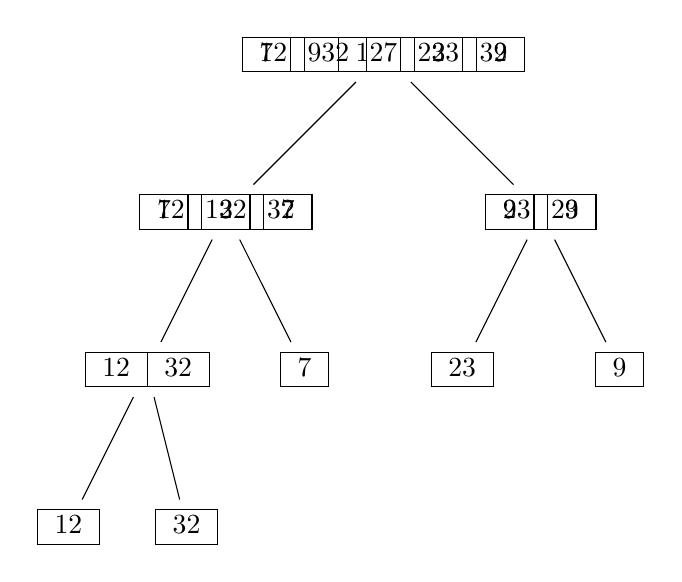
\begin{tikzpicture}

\uncover<1-8>{
\node (t) at (0,0) {\begin{tabular}{|c|c|c|c|c|}
\hline
12 & 32 & 7 & 23 & 9 \\
\hline
\end{tabular}};
}

\uncover<2-5>{
\node (t1) at (-2, -2) {\begin{tabular}{|c|c|c|}
\hline
12 & 32 & 7 \\
\hline
\end{tabular}};
}

\uncover<3-5>{
\node (t11) at (-3, -4) {\begin{tabular}{|c|c|}
\hline
12 & 32 \\
\hline
\end{tabular}};

\node (t12) at (-1, -4) {\begin{tabular}{|c|}
\hline
7 \\
\hline
\end{tabular}};
}

\uncover<4>{
\node (t111) at (-4, -6) {\begin{tabular}{|c|}
\hline
12 \\
\hline
\end{tabular}};

\node (t112) at (-2.5, -6) {\begin{tabular}{|c|}
\hline
32 \\
\hline
\end{tabular}};
}

\uncover<6-8>{
\node (t1) at (-2, -2) {\begin{tabular}{|c|c|c|}
\hline
7 & 12 & 32 \\
\hline
\end{tabular}};
}


\uncover<2-7>{
\node (t2) at (2, -2) {\begin{tabular}{|c|c|}
\hline
23 & 9 \\
\hline
\end{tabular}};
}

\uncover<7>{
\node (t21) at (1, -4) {\begin{tabular}{|c|}
\hline
23\\
\hline
\end{tabular}};

\node (t22) at (3, -4) {\begin{tabular}{|c|}
\hline
9\\
\hline
\end{tabular}};
}

\uncover<8>{
\node (t2) at (2, -2) {\begin{tabular}{|c|c|}
\hline
9 & 23 \\
\hline
\end{tabular}};
}

\uncover<9>{
\node (t) at (0,0) {\begin{tabular}{|c|c|c|c|c|}
\hline
7 & 9 & 12 & 23 & 32 \\
\hline
\end{tabular}};
}

\uncover<2-8>{
\draw (t) -- (t1);
\draw (t) -- (t2);
}

\uncover<3-5>{
\draw (t1) -- (t11);
\draw (t1) -- (t12);
}

\uncover<4>{
\draw (t11) -- (t111);
\draw (t11) -- (t112);
}

\uncover<7>{
\draw (t2) -- (t21);
\draw (t2) -- (t22);
}

\end{tikzpicture}

}

\frame{
\frametitle{Le tri fusion~: caractéristiques}

\begin{block}{Stable}
Le tri fusion peut être implanté de façon à être stable.
\end{block}

\begin{block}{En place}
Avec un surcoût en nombre d'opérations dans le pire cas.
\end{block}

\begin{columns}
\begin{column}{5cm}
\begin{block}{Opérations dans le pire cas}
De l'ordre de $len(t)\log(len(t))$.
\end{block}
\end{column}
\begin{column}{5cm}
\begin{block}{Opérations en moyenne}
De l'ordre de $len(t)\log(len(t))$.
\end{block}
\end{column}
\end{columns}

\vfill

\begin{alertblock}{Approche diviser pour régner}
Séparation d'un problème en sous-problèmes plus petits, combinaison des solutions à ces problèmes.
\end{alertblock}

}

\frame{
\frametitle{Le tri rapide~: principe}

\begin{block}{Approche diviser pour régner}
  \begin{itemize}
    \item Choisir un élément $p$ de $t$, qu'on appelle pivot,
    \item Diviser le tableau $t$ à trier en deux tableaux $t1$ et $t2$ tels que tous les éléments de $t1$ sont plus petits que $p$ et tous les éléments de $t2$ sont plus grands que $p$,
    \item Trier $t1$ et $t2$ (éventuellement de la même façon),
    \item Mettre $t1$ et $t2$ bout à bout pour obtenir une version triée du tableau $t$.
  \end{itemize}
  \alert{En pratique ceci se fait en place, $t1$ et $t2$ sont stockés dans $t$, de part et d'autre de $p$.}
\end{block}

\begin{block}{Un exemple en dansant}
\url{https://www.youtube.com/watch?v=ywWBy6J5gz8}
\end{block}

}

\frame{
\frametitle{Le tri rapide~: algorithme}

\begin{alertblock}{Tri rapide de $t[p:r]$}
Si $len(t[p:r]) > 1$, alors $q = partitionner(t[p:r])$, puis faire le tri rapide de $t[p:q]$ et de $t[q+1:r]$.
\end{alertblock}

\begin{alertblock}{Partitionner($t[p:r]$)}
Soit $pivot = t[p]$, soit $i=p$, soit $j=r-1$.\\
Tant que $i < j$ faire,\\
~~~~~~~~tant que $t[j] \geq pivot$ et $i < j$, diminuer $j$ de 1;\\
~~~~~~~~si $i<j$, inverser $t[i]$ et $t[j]$;\\
~~~~~~~~tant que $t[i] \leq pivot$ et $i < j$, augmenter $i$ de 1;\\
~~~~~~~~si $i<j$, inverser $t[i]$ et $t[j]$.\\
Retourner $i$.
\end{alertblock}

}

\frame{
\frametitle{Le tri rapide~: exemple}

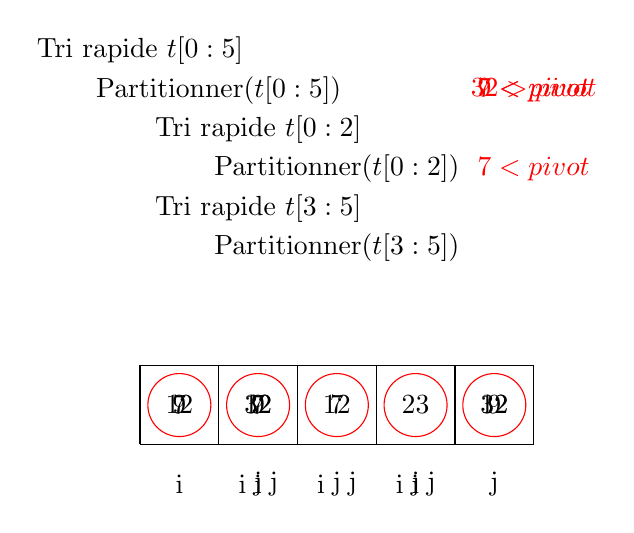
\begin{tikzpicture}

\node (app) at (0,5) {Tri rapide $t[0:5]$};
\uncover<2->{\node (app) at (1,4.5) {Partitionner($t[0:5]$)};}
\uncover<4>{\node (info) at (5,4.5) {\textcolor{red}{$9 < pivot$}};}
\uncover<7>{\node (info) at (5,4.5) {\textcolor{red}{$32 > pivot$}};}
\uncover<11>{\node (info) at (5,4.5) {\textcolor{red}{$7 < pivot$}};}
\uncover<14->{\node (app) at (1.5,4) {Tri rapide $t[0:2]$};}
\uncover<15->{\node (app) at (2.5,3.5) {Partitionner($t[0:2]$)};}
\uncover<16>{\node (info) at (5,3.5) {\textcolor{red}{$7 < pivot$}};}
\uncover<14->{\node (app) at (1.5,3) {Tri rapide $t[3:5]$};}
\uncover<19-21>{\node (app) at (2.5,2.5) {Partitionner($t[3:5]$)};}

\draw (0,0) -- (5,0) -- (5,1) -- (0,1) -- (0,0);
\draw (1,0) -- (1,1);
\draw (2,0) -- (2,1);
\draw (3,0) -- (3,1);
\draw (4,0) -- (4,1);
\uncover<1-4>{
\node (a) at (0.5,0.5) {12};
}
\uncover<5-16>{
\node (a) at (0.5,0.5) {9};
}
\uncover<17->{
\node (a) at (0.5,0.5) {7};
}
\uncover<1-7>{
\node (b) at (1.5,0.5) {32};
}
\uncover<8-11>{
\node (b) at (1.5,0.5) {12};
}
\uncover<12-16>{
\node (b) at (1.5,0.5) {7};
}
\uncover<17->{
\node (b) at (1.5,0.5) {9};
}
\uncover<1-11>{
\node (c) at (2.5,0.5) {7};
}
\uncover<12->{
\node (c) at (2.5,0.5) {12};
}
\node (d) at (3.5,0.5) {23};
\uncover<1-4>{
\node (e) at (4.5,0.5) {9};
}
\uncover<5-7>{
\node (e) at (4.5,0.5) {12};
}
\uncover<8->{
\node (e) at (4.5,0.5) {32};
}

\uncover<3-5,15-17>{
\node (i) at (0.5,-0.5) {i};
}
\uncover<6-12>{
\node (i) at (1.5,-0.5) {i};
}
\uncover<13>{
\node (i) at (2.3,-0.5) {i};
}
\uncover<18>{
\node (i) at (1.3,-0.5) {i};
}
\uncover<19>{
\node (i) at (3.5,-0.5) {i};
}
\uncover<20>{
\node (i) at (3.3,-0.5) {i};
}

\uncover<3-8,19>{
\node (j) at (4.5,-0.5) {j};
}
\uncover<9>{
\node (j) at (3.5,-0.5) {j};
}
\uncover<20>{
\node (j) at (3.7,-0.5) {j};
}
\uncover<10-12>{
\node (j) at (2.5,-0.5) {j};
}
\uncover<13>{
\node (j) at (2.7,-0.5) {j};
}
\uncover<15-17>{
\node (j) at (1.5,-0.5) {j};
}
\uncover<18>{
\node (j) at (1.7,-0.5) {j};
}

\uncover<3-4,15-16>{
\node[minimum size=0.8cm,draw=red,circle] (pivot) at (0.5,0.5) {};
}
\uncover<5-7>{
\node[minimum size=0.8cm,draw=red,circle] (pivot) at (4.5,0.5) {};
}
\uncover<8-11,17-18>{
\node[minimum size=0.8cm,draw=red,circle] (pivot) at (1.5,0.5) {};
}
\uncover<12-13>{
\node[minimum size=0.8cm,draw=red,circle] (pivot) at (2.5,0.5) {};
}
\uncover<19-20>{
\node[minimum size=0.8cm,draw=red,circle] (pivot) at (3.5,0.5) {};
}


\end{tikzpicture}

}

\frame{
\frametitle{Le tri rapide~: caractéristiques}


\begin{block}{Pas stable}
Le tri rapide n'est pas stable.
\end{block}

\begin{block}{En place}
Le tri rapide est effectué en place.
\end{block}

\begin{columns}
\begin{column}{5cm}
\begin{block}{Opérations dans le pire cas}
De l'ordre de $len(t)^2$.
\end{block}
\end{column}
\begin{column}{5cm}
\begin{block}{Opérations en moyenne}
De l'ordre de $len(t)\log(len(t))$.
\end{block}
\end{column}
\end{columns}

\vfill

\begin{alertblock}{Efficace en pratique}
En pratique le pire cas est rarement atteint et les coefficients du nombre d'opérations en moyenne sont petits par rapport aux autres tris, ce qui fait qu'on préfère souvent le tri rapide.
\end{alertblock}

}


\end{document}
